\documentclass{standalone}
\usepackage{tikz}
\usetikzlibrary{patterns, positioning}

\begin{document}
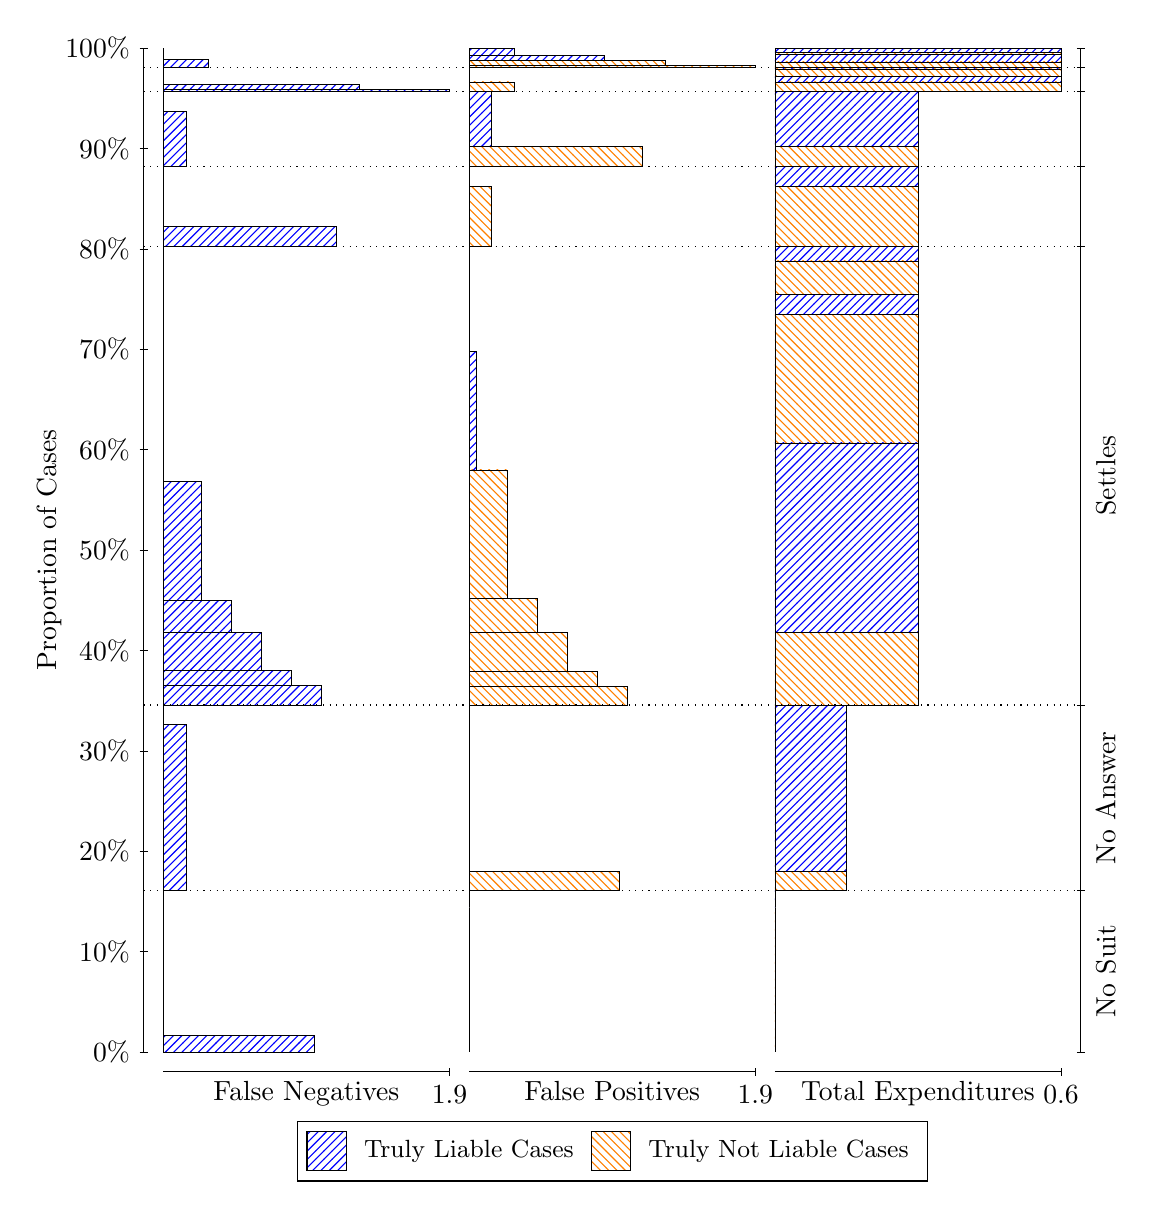
\begin{tikzpicture}
\draw[black, very thin] (1.5,1.75) -- (1.5,14.5);
\node[rotate=90, anchor=center] at (0.3, 8.125) {Proportion of Cases};
\draw[black, very thin] (1.45,1.75) -- (1.55,1.75);
\node[anchor=east] at (1.45, 1.75) {0\%};
\draw[black, very thin] (1.45,3.025) -- (1.55,3.025);
\node[anchor=east] at (1.45, 3.025) {10\%};
\draw[black, very thin] (1.45,4.3) -- (1.55,4.3);
\node[anchor=east] at (1.45, 4.3) {20\%};
\draw[black, very thin] (1.45,5.575) -- (1.55,5.575);
\node[anchor=east] at (1.45, 5.575) {30\%};
\draw[black, very thin] (1.45,6.85) -- (1.55,6.85);
\node[anchor=east] at (1.45, 6.85) {40\%};
\draw[black, very thin] (1.45,8.125) -- (1.55,8.125);
\node[anchor=east] at (1.45, 8.125) {50\%};
\draw[black, very thin] (1.45,9.4) -- (1.55,9.4);
\node[anchor=east] at (1.45, 9.4) {60\%};
\draw[black, very thin] (1.45,10.675) -- (1.55,10.675);
\node[anchor=east] at (1.45, 10.675) {70\%};
\draw[black, very thin] (1.45,11.95) -- (1.55,11.95);
\node[anchor=east] at (1.45, 11.95) {80\%};
\draw[black, very thin] (1.45,13.225) -- (1.55,13.225);
\node[anchor=east] at (1.45, 13.225) {90\%};
\draw[black, very thin] (1.45,14.5) -- (1.55,14.5);
\node[anchor=east] at (1.45, 14.5) {100\%};

\draw[black, very thin] (13.4,1.75) -- (13.4,14.5);
\draw[black, very thin] (13.35,1.75) -- (13.45,1.75);
\node[anchor=west] at (13.35, 1.75) {};
\draw[black, very thin] (13.35,3.799) -- (13.45,3.799);
\node[anchor=west] at (13.35, 3.799) {};
\draw[black, very thin] (13.35,6.1565) -- (13.45,6.1565);
\node[anchor=west] at (13.35, 6.1565) {};
\draw[black, very thin] (13.35,11.985) -- (13.45,11.985);
\node[anchor=west] at (13.35, 11.985) {};
\draw[black, very thin] (13.35,12.994) -- (13.45,12.994);
\node[anchor=west] at (13.35, 12.994) {};
\draw[black, very thin] (13.35,13.953) -- (13.45,13.953);
\node[anchor=west] at (13.35, 13.953) {};
\draw[black, very thin] (13.35,14.256) -- (13.45,14.256);
\node[anchor=west] at (13.35, 14.256) {};
\draw[black, very thin] (13.35,14.5) -- (13.45,14.5);
\node[anchor=west] at (13.35, 14.5) {};

\draw[black, very thin, pattern color=blue, pattern=north east lines] (1.75,1.75) rectangle (3.6623,1.9656);
\draw[black, very thin, pattern color=orange, pattern=north west lines] (1.75,1.9656) rectangle (1.75,3.799);
\draw[black, very thin, pattern color=blue, pattern=north east lines] (1.75,3.799) rectangle (2.0368,5.9143);
\draw[black, very thin, pattern color=orange, pattern=north west lines] (1.75,5.9143) rectangle (1.75,6.1565);
\draw[black, very thin, pattern color=blue, pattern=north east lines] (1.75,6.1565) rectangle (3.7579,6.4058);
\draw[black, very thin, pattern color=blue, pattern=north east lines] (1.75,6.4058) rectangle (3.3754,6.5946);
\draw[black, very thin, pattern color=blue, pattern=north east lines] (1.75,6.5946) rectangle (3.1842,6.5956);
\draw[black, very thin, pattern color=blue, pattern=north east lines] (1.75,6.5956) rectangle (2.993,7.0813);
\draw[black, very thin, pattern color=blue, pattern=north east lines] (1.75,7.0813) rectangle (2.8018,7.0818);
\draw[black, very thin, pattern color=blue, pattern=north east lines] (1.75,7.0818) rectangle (2.6105,7.4895);
\draw[black, very thin, pattern color=blue, pattern=north east lines] (1.75,7.4895) rectangle (2.4193,7.49);
\draw[black, very thin, pattern color=blue, pattern=north east lines] (1.75,7.49) rectangle (2.2281,9);
\draw[black, very thin, pattern color=orange, pattern=north west lines] (1.75,9) rectangle (1.75,11.985);
\draw[black, very thin, pattern color=blue, pattern=north east lines] (1.75,11.985) rectangle (3.9491,12.236);
\draw[black, very thin, pattern color=orange, pattern=north west lines] (1.75,12.236) rectangle (1.75,12.994);
\draw[black, very thin, pattern color=blue, pattern=north east lines] (1.75,12.994) rectangle (2.0368,13.699);
\draw[black, very thin, pattern color=orange, pattern=north west lines] (1.75,13.699) rectangle (1.75,13.953);
\draw[black, very thin, pattern color=blue, pattern=north east lines] (1.75,13.953) rectangle (5.3833,13.974);
\draw[black, very thin, pattern color=blue, pattern=north east lines] (1.75,13.974) rectangle (4.236,14.042);
\draw[black, very thin, pattern color=orange, pattern=north west lines] (1.75,14.042) rectangle (1.75,14.256);
\draw[black, very thin, pattern color=blue, pattern=north east lines] (1.75,14.256) rectangle (2.3237,14.352);
\draw[black, very thin, pattern color=orange, pattern=north west lines] (1.75,14.352) rectangle (1.75,14.44);
\draw[black, very thin, pattern color=blue, pattern=north east lines] (1.75,14.44) rectangle (1.75,14.5);
\draw[black, very thin, pattern color=orange, pattern=north west lines] (5.6333,1.75) rectangle (5.6333,3.5835);
\draw[black, very thin, pattern color=blue, pattern=north east lines] (5.6333,3.5835) rectangle (5.6333,3.799);
\draw[black, very thin, pattern color=orange, pattern=north west lines] (5.6333,3.799) rectangle (7.5456,4.0412);
\draw[black, very thin, pattern color=blue, pattern=north east lines] (5.6333,4.0412) rectangle (5.6333,6.1565);
\draw[black, very thin, pattern color=orange, pattern=north west lines] (5.6333,6.1565) rectangle (7.6412,6.3964);
\draw[black, very thin, pattern color=orange, pattern=north west lines] (5.6333,6.3964) rectangle (7.45,6.3974);
\draw[black, very thin, pattern color=orange, pattern=north west lines] (5.6333,6.3974) rectangle (7.2588,6.583);
\draw[black, very thin, pattern color=orange, pattern=north west lines] (5.6333,6.583) rectangle (7.0675,6.584);
\draw[black, very thin, pattern color=orange, pattern=north west lines] (5.6333,6.584) rectangle (6.8763,7.076);
\draw[black, very thin, pattern color=orange, pattern=north west lines] (5.6333,7.076) rectangle (6.6851,7.0809);
\draw[black, very thin, pattern color=orange, pattern=north west lines] (5.6333,7.0809) rectangle (6.4939,7.5089);
\draw[black, very thin, pattern color=orange, pattern=north west lines] (5.6333,7.5089) rectangle (6.1114,9.1411);
\draw[black, very thin, pattern color=blue, pattern=north east lines] (5.6333,9.1411) rectangle (5.7289,10.651);
\draw[black, very thin, pattern color=blue, pattern=north east lines] (5.6333,10.651) rectangle (5.6333,11.985);
\draw[black, very thin, pattern color=orange, pattern=north west lines] (5.6333,11.985) rectangle (5.9202,12.743);
\draw[black, very thin, pattern color=blue, pattern=north east lines] (5.6333,12.743) rectangle (5.6333,12.994);
\draw[black, very thin, pattern color=orange, pattern=north west lines] (5.6333,12.994) rectangle (7.8325,13.248);
\draw[black, very thin, pattern color=blue, pattern=north east lines] (5.6333,13.248) rectangle (5.9202,13.953);
\draw[black, very thin, pattern color=orange, pattern=north west lines] (5.6333,13.953) rectangle (6.207,14.069);
\draw[black, very thin, pattern color=orange, pattern=north west lines] (5.6333,14.069) rectangle (5.6333,14.167);
\draw[black, very thin, pattern color=blue, pattern=north east lines] (5.6333,14.167) rectangle (5.6333,14.256);
\draw[black, very thin, pattern color=orange, pattern=north west lines] (5.6333,14.256) rectangle (9.2667,14.275);
\draw[black, very thin, pattern color=orange, pattern=north west lines] (5.6333,14.275) rectangle (8.1193,14.344);
\draw[black, very thin, pattern color=blue, pattern=north east lines] (5.6333,14.344) rectangle (7.3544,14.404);
\draw[black, very thin, pattern color=blue, pattern=north east lines] (5.6333,14.404) rectangle (6.207,14.5);
\draw[black, very thin, pattern color=orange, pattern=north west lines] (9.5167,1.75) rectangle (9.5167,3.5835);
\draw[black, very thin, pattern color=blue, pattern=north east lines] (9.5167,3.5835) rectangle (9.5167,3.799);
\draw[black, very thin, pattern color=orange, pattern=north west lines] (9.5167,3.799) rectangle (10.425,4.0412);
\draw[black, very thin, pattern color=blue, pattern=north east lines] (9.5167,4.0412) rectangle (10.425,6.1565);
\draw[black, very thin, pattern color=orange, pattern=north west lines] (9.5167,6.1565) rectangle (11.333,7.0809);
\draw[black, very thin, pattern color=blue, pattern=north east lines] (9.5167,7.0809) rectangle (11.333,9.4863);
\draw[black, very thin, pattern color=orange, pattern=north west lines] (9.5167,9.4863) rectangle (11.333,11.119);
\draw[black, very thin, pattern color=blue, pattern=north east lines] (9.5167,11.119) rectangle (11.333,11.368);
\draw[black, very thin, pattern color=orange, pattern=north west lines] (9.5167,11.368) rectangle (11.333,11.796);
\draw[black, very thin, pattern color=blue, pattern=north east lines] (9.5167,11.796) rectangle (11.333,11.985);
\draw[black, very thin, pattern color=orange, pattern=north west lines] (9.5167,11.985) rectangle (11.333,12.743);
\draw[black, very thin, pattern color=blue, pattern=north east lines] (9.5167,12.743) rectangle (11.333,12.994);
\draw[black, very thin, pattern color=orange, pattern=north west lines] (9.5167,12.994) rectangle (11.333,13.248);
\draw[black, very thin, pattern color=blue, pattern=north east lines] (9.5167,13.248) rectangle (11.333,13.953);
\draw[black, very thin, pattern color=orange, pattern=north west lines] (9.5167,13.953) rectangle (13.15,14.069);
\draw[black, very thin, pattern color=blue, pattern=north east lines] (9.5167,14.069) rectangle (13.15,14.136);
\draw[black, very thin, pattern color=orange, pattern=north west lines] (9.5167,14.136) rectangle (13.15,14.234);
\draw[black, very thin, pattern color=blue, pattern=north east lines] (9.5167,14.234) rectangle (13.15,14.256);
\draw[black, very thin, pattern color=orange, pattern=north west lines] (9.5167,14.256) rectangle (13.15,14.325);
\draw[black, very thin, pattern color=blue, pattern=north east lines] (9.5167,14.325) rectangle (13.15,14.421);
\draw[black, very thin, pattern color=orange, pattern=north west lines] (9.5167,14.421) rectangle (13.15,14.44);
\draw[black, very thin, pattern color=blue, pattern=north east lines] (9.5167,14.44) rectangle (13.15,14.5);
\draw[black, dotted] (1.5,3.799) -- (13.4,3.799);
\draw[black, dotted] (1.5,6.1565) -- (13.4,6.1565);
\draw[black, dotted] (1.5,11.985) -- (13.4,11.985);
\draw[black, dotted] (1.5,12.994) -- (13.4,12.994);
\draw[black, dotted] (1.5,13.953) -- (13.4,13.953);
\draw[black, dotted] (1.5,14.256) -- (13.4,14.256);
\draw[black, very thin] (1.75,1.5) -- (5.3833,1.5);
\node[anchor=north] at (3.5667, 1.5) {False Negatives};
\draw[black, very thin] (5.3833,1.45) -- (5.3833,1.55);
\node[anchor=north] at (5.3833, 1.45) {1.9};

\draw[black, very thin] (5.6333,1.5) -- (9.2667,1.5);
\node[anchor=north] at (7.45, 1.5) {False Positives};
\draw[black, very thin] (9.2667,1.45) -- (9.2667,1.55);
\node[anchor=north] at (9.2667, 1.45) {1.9};

\draw[black, very thin] (9.5167,1.5) -- (13.15,1.5);
\node[anchor=north] at (11.333, 1.5) {Total Expenditures};
\draw[black, very thin] (13.15,1.45) -- (13.15,1.55);
\node[anchor=north] at (13.15, 1.45) {0.6};

\node[black, centered, rotate=90] at (13.72, 2.7745) {No Suit};
\node[black, centered, rotate=90] at (13.72, 4.9777) {No Answer};
\node[black, centered, rotate=90] at (13.72, 9.0706) {Settles};





\draw (7.449999999999999,1.5) node[draw=none] (baseCoordinate) {};
\begin{scope}[align=center]
        \matrix[scale=0.5, draw=black, below=0.5cm of baseCoordinate, nodes={draw}, column sep=0.1cm]{
            \node[rectangle, draw, minimum width=0.5cm, minimum height=0.5cm, pattern=north east lines, pattern color=blue] {}; &
            \node[draw=none, font=\small] (B) {Truly Liable Cases}; &
            \node[rectangle, draw, minimum width=0.5cm, minimum height=0.5cm, pattern=north west lines, pattern color=orange] {}; &
            \node[draw=none, font=\small] (B) {Truly Not Liable Cases}; \\
            };
\end{scope}

\end{tikzpicture}
\end{document}